\documentclass{article}
\usepackage{amsmath, amsthm, amsfonts}
\usepackage{centernot}
\usepackage{caption}
\usepackage{tikz}
\usetikzlibrary{automata, positioning, arrows}
\tikzset{
->, % makes the edges directed
>=stealth', % makes the arrow heads bold
node distance=3cm, % specifies the minimum distance between two nodes. Change if necessary.
every state/.style={thick, fill=gray!10}, % sets the properties for each ’state’ node
initial text=$ $, % sets the text that appears on the start arrow
}
\usepackage{float}
\author{Mostafa Hassanein}
\title{
  MTH-682 Automata \\
  Assignment (2): Context-Free Languages}
\date{20 November 2025}
\begin{document}
\maketitle
\newpage

\section*{2.1}

Recall the CFG G4 that we gave in Example 2.4. For convenience, let's rename its variables with single letters as follows.
\begin{align*}
  E &\rightarrow E + T | T \\
  T &\rightarrow T x F | F \\
  F &\rightarrow (E) | a \\
\end{align*}
Give parse trees and derivations for each string.

\subsection*{c. $a+a+a$}

\begin{center}
  \underline{Solution:}
\end{center}

\noindent
\begin{minipage}[t]{0.45\textwidth}
\textbf{Derivation:}

We derive the string $a+a+a$ from the start symbol $E$ as follows:

\begin{align*}
  E &\Rightarrow E + T \\
  &\Rightarrow E + T + T \\
  &\Rightarrow T + T + T \\
  &\Rightarrow F + T + T \\
  &\Rightarrow a + T + T \\
  &\Rightarrow a + F + T \\
  &\Rightarrow a + a + T \\
  &\Rightarrow a + a + F \\
  &\Rightarrow a + a + a
\end{align*}
\end{minipage}
\hspace{0.5cm}
\vrule
\hspace{0.5cm}
\begin{minipage}[t]{0.5\textwidth}
\textbf{Parse Tree:}

\begin{center}
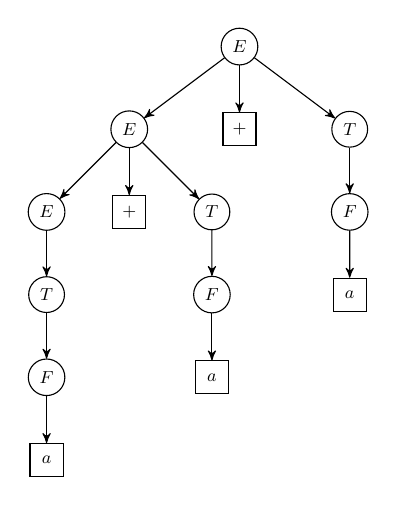
\begin{tikzpicture}[
  scale=0.7,
  transform shape,
  level 1/.style={sibling distance=2cm},
  level 2/.style={sibling distance=1.5cm},
  level 3/.style={sibling distance=1cm},
  level 4/.style={sibling distance=0.7cm},
  every node/.style={circle, draw, minimum size=0.6cm, font=\small}
]
  \node {$E$}
    child {node {$E$}
      child {node {$E$}
        child {node {$T$}
          child {node {$F$}
            child {node[rectangle] {$a$}}
          }
        }
      }
      child {node[rectangle] {$+$}}
      child {node {$T$}
        child {node {$F$}
          child {node[rectangle] {$a$}}
        }
      }
    }
    child {node[rectangle] {$+$}}
    child {node {$T$}
      child {node {$F$}
        child {node[rectangle] {$a$}}
      }
    };
\end{tikzpicture}
\end{center}
\end{minipage}

\subsection*{c. $((a))$}

\begin{center}
  \underline{Solution:}
\end{center}

\noindent
\begin{minipage}[t]{0.45\textwidth}
\textbf{Derivation:}

We derive the string $((a))$ from the start symbol $E$ as follows:

\begin{align*}
  E &\Rightarrow T \\
  &\Rightarrow F \\
  &\Rightarrow (E) \\
  &\Rightarrow (T) \\
  &\Rightarrow (F) \\
  &\Rightarrow ((E)) \\
  &\Rightarrow ((T)) \\
  &\Rightarrow ((F)) \\
  &\Rightarrow ((a))
\end{align*}
\end{minipage}
\hspace{0.5cm}
\vrule
\hspace{0.5cm}
\begin{minipage}[t]{0.5\textwidth}
\textbf{Parse Tree:}

\begin{center}
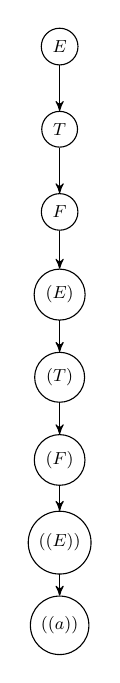
\begin{tikzpicture}[
  scale=0.7,
  transform shape,
  level 1/.style={sibling distance=2cm},
  level 2/.style={sibling distance=1.5cm},
  level 3/.style={sibling distance=1cm},
  level 4/.style={sibling distance=0.7cm},
  every node/.style={circle, draw, minimum size=0.6cm, font=\small}
]
  \node {$E$}
    child {node {$T$}
      child {node {$F$}
        child {node {$(E)$}
          child {node {$(T)$}
            child {node {$(F)$}
              child {node {$((E))$}
                child {node {$((a))$}
                }
              }
            }
          }
        }
      }
    };
\end{tikzpicture}
\end{center}
\end{minipage}
\newpage

\section*{2.4}
Give context-free grammars that generate the following languages. In all parts, the alphabet $\Sigma$ is $\{0,1\}$.

\subsection*{c. $\{w| \text{ the length of w is odd}\}$}

\begin{center}
  \underline{Solution:}
\end{center}

\begin{align*}
  S &\rightarrow ASA | 0 | 1 \\
  A &\rightarrow 0 | 1
\end{align*}

\subsection*{c. The empty set}
\begin{center}
  \underline{Solution:}
\end{center}
\begin{align*}
  S &\rightarrow S
\end{align*}

This language has a single rule that infinitely recurses and never terminates to any terminal symbols. Therefore, no words belong to this language.
\newpage

\section*{2.5}
Give informal descriptions and state diagrams of pushdown automata for the languages in Exercise 2.4.

\subsection*{c. $\{w| \text{ the length of w is odd}\}$}

\begin{center}
  \underline{Solution:}
\end{center}

\textbf{Informal Description:}

The pushdown automaton reads input symbols (0 or 1) one at a time and uses two states to track the parity of the number of symbols read. It starts in state $q_0$ (representing an even count, since 0 symbols have been read). Each input symbol causes a transition that toggles between states $q_0$ and $q_1$. After reading all input, if the automaton is in state $q_1$ (odd count), it transitions to the accept state $q_{accept}$.

The stack is not essential for this language, but we include it for the formal PDA definition. We use a bottom-of-stack marker \$ to detect when input is complete.

\vspace{0.5cm}

\textbf{State Diagram:}

\begin{center}
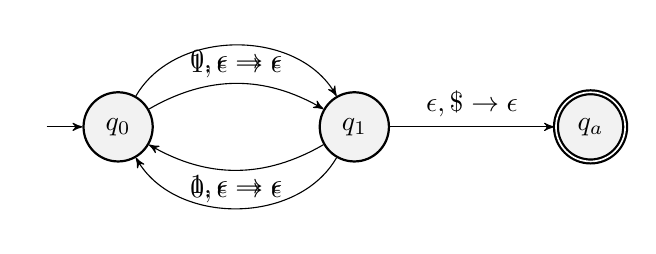
\begin{tikzpicture}[node distance=3cm, auto]
  % States
  \node[state, initial] (q0) {$q_0$};
  \node[state, right of=q0] (q1) {$q_1$};
  \node[state, accepting, right of=q1] (qa) {$q_a$};

  % Transitions
  \path[->]
    (q0) edge[bend left] node[above] {$0,\epsilon\rightarrow\epsilon$} (q1)
    (q0) edge[bend left=60] node[below] {$1,\epsilon\rightarrow\epsilon$} (q1)
    (q1) edge[bend left] node[below] {$0,\epsilon\rightarrow\epsilon$} (q0)
    (q1) edge[bend left=60] node[above] {$1,\epsilon\rightarrow\epsilon$} (q0)
    (q1) edge node[above] {$\epsilon,\$\rightarrow\epsilon$} (qa);
\end{tikzpicture}
\end{center}

\vspace{0.3cm}

\textbf{Formal Description:}
\begin{itemize}
  \item States: $Q = \{q_0, q_1, q_a\}$
  \item Start state: $q_0$
  \item Accept state: $q_a$
  \item Stack alphabet: $\Gamma = \{\$\}$
  \item Initial stack symbol: \$
  \item Transitions:
  \begin{align*}
    \delta(q_0, 0, \epsilon) &= \{(q_1, \epsilon)\} \\
    \delta(q_0, 1, \epsilon) &= \{(q_1, \epsilon)\} \\
    \delta(q_1, 0, \epsilon) &= \{(q_0, \epsilon)\} \\
    \delta(q_1, 1, \epsilon) &= \{(q_0, \epsilon)\} \\
    \delta(q_1, \epsilon, \$) &= \{(q_a, \epsilon)\}
  \end{align*}
\end{itemize}

The automaton alternates between states $q_0$ and $q_1$ for each symbol read. It accepts if and only if it ends in state $q_1$ (odd number of symbols) and can transition to $q_a$ by popping the bottom marker \$.


\subsection*{f.}

\begin{center}
  \underline{Solution:}
\end{center}

\newpage

\section*{2.11}
Convert the CFG G4 given in Exercise 2.1 to an equivalent PDA, using the procedure
given in Theorem 2.20.

\begin{center}
  \underline{Solution:}
\end{center}

\newpage

\section*{2.13}

Let $G = (V, \Sigma, R, S)$ be the following grammar. $V = {S, T, U};$ $\Sigma = {0, \#};$ and
$R$ is the set of rules:

\begin{align*}
  S &\rightarrow TT | U \\
  T &\rightarrow 0T | T0 | \# \\
  U &\rightarrow 0U00 | \#
\end{align*}

a. Describe $L(G)$ in English.

b. Prove that $L(G)$ is not regular.

\subsection*{a.}

\begin{center}
  \underline{Solution:}
\end{center}

\subsection*{b.}

\begin{center}
  \underline{Solution:}
\end{center}

\newpage

\section*{2.14}
Convert the following CFG into an equivalent CFG in Chomsky normal form,
using the procedure given in Theorem 2.9.
\begin{align*}
  A &\rightarrow BAB | B | \epsilon \\
  B &\rightarrow 00 | \epsilon
\end{align*}

\begin{center}
  \underline{Solution:}
\end{center}

\newpage

\section*{2.23}
Let $D = \{xy| \: x, y \in \{0,1\}^*$ and $|x| = |y|$ but $x \neq y\}$.

\noindent
Show that D is a context-free language.

\begin{center}
  \underline{Solution:}
\end{center}

\newpage

\section*{2.24}
Let $E = \{a^ib^j| \: i \neq j$ and $2i \neq j\}$.

\noindent
Show that E is a context-free language.

\begin{center}
  \underline{Solution:}
\end{center}

\newpage

\section*{2.26}
Show that if G is a CFG in Chomsky normal form, then for any string $w \in L(G)$
of length n $n \geq 1$, exactly $2n-1$ steps are required for any derivation of w.

\begin{center}
  \underline{Solution:}
\end{center}

\newpage

\section*{2.27}

Let $G = (V, \Sigma ,R, <STMT>)$ be the following grammar.
\begin{align*}
  <STMT> &\rightarrow <ASSIGN> | <IF-THEN> | <IF-THEN-ELSE> \\
  <IF-THEN> &\rightarrow if condition then <STMT> \\
  <IF-THEN-ELSE> &\rightarrow if condition then <STMT> else <STMT> \\
  <ASSIGN> &\rightarrow a:=1
\end{align*}

$\Sigma = \{if, \: condition, \: then, \: else, \: a:=1\}$

$V = \{<STMT>, \: <IF-THEN>, \: <IF-ELSE-THEN>, \: <ASSIGN>\}$
\newline

\noindent
G is a natural-looking grammar for a fragment of a programming language, but G
is ambiguous.
\newline

a. Show that G is ambiguous.

b. Give a new unambiguous grammar for the same language.

\subsection*{a.}

\begin{center}
  \underline{Solution:}
\end{center}

\subsection*{b.}

\begin{center}
  \underline{Solution:}
\end{center}

\newpage

\section*{30}
Use the pumping lemma to show that the following languages are not context free.

\subsection*{d.}
\begin{align*}
  L = \Bigl\{t1\#t2\# \ldots \#t_k| \: k \geq 2, \forall i \: t_i \in \{a, b\}^* \: \land \: \exists i,j: (t_i = t_j \: \land \: i \neq j)\Bigr\}
\end{align*}

\begin{center}
  \underline{Solution:}
\end{center}

\newpage

\section*{2.31}
Let B be the language of all palindromes over $\{0,1\}$ containing equal numbers of
0s and 1s. Show that B is not context free.

\begin{center}
  \underline{Solution:}
\end{center}


\end{document}